% =========================================================
% RESULTADOS E DISCUSSÃO
% FINALIDADE: apresentar os resultados e interpretá-los à luz da
%   fundamentação teórica.
% ESCREVA: os resultados em sequência lógica (por exemplo, por objetivo
%   específico), seguidos da discussão.
% CUIDADO: cite e comente cada tabela ou ilustração no texto.
% EXEMPLOS NESTE ARQUIVO: tabela, gráfico e equação.
% Os dados dos exemplos são fictícios e devem ser substituídos.
% Resultados e discussão podem ser apresentados em seções primárias
% separadas, conforme a orientação.
% =========================================================

\chapter{RESULTADOS E DISCUSSÃO}
\label{cap:resultados}

Nesta seção, apresentam-se os resultados da pesquisa e sua discussão à luz da fundamentação teórica. Recomenda-se organizar as seções de acordo com os objetivos específicos, de modo que cada um deles seja retomado de forma explícita.

\section{Resultados referentes ao primeiro objetivo específico}
\label{sec:resultado1}

Os resultados devem ser apresentados com objetividade, em sequência lógica, e acompanhados da interpretação do(a) autor(a). Tabelas e ilustrações complementam o texto, mas não o substituem: toda tabela ou ilustração deve ser citada e comentada antes de sua apresentação, como na Tabela~\ref{tab:exemplo}.

% Exemplo de tabela (padrão IBGE e modelo BCZM/UFRN): sem bordas
% laterais; traços horizontais no topo, no cabeçalho e no fechamento;
% traços verticais apenas entre as colunas.
% Em cada linha, & separa as células e \\ encerra a linha.
% \titulocoluna{...} deixa o cabeçalho em negrito e centralizado.
\begin{table}[htbp]
\begin{ilustracao}{0.7\linewidth}
\caption{Distribuição dos participantes por categoria}
\label{tab:exemplo}
\begin{tabularx}{\linewidth}{X|c|c}
\hline
\titulocoluna{Categoria} & \titulocoluna{Frequência} & \titulocoluna{Percentual (\%)} \\
\hline
Categoria A & 12 & 25,0 \\
Categoria B & 18 & 37,5 \\
Categoria C & 10 & 20,8 \\
Categoria D &  8 & 16,7 \\
\hline
Total       & 48 & 100,0 \\
\hline
\end{tabularx}
\fonte{Elaboração própria (\ano). Dados fictícios.}
\end{ilustracao}
\end{table}

O Gráfico~\ref{gra:exemplo} apresenta os mesmos dados em forma de barras. Gráficos produzidos em outros programas devem ser exportados preferencialmente em PDF ou em PNG de alta resolução.

% Exemplo de gráfico. O ambiente grafico gera a Lista de Gráficos.
% Troque exemplo-grafico.pdf pelo nome do seu arquivo (PDF, PNG ou JPG
% salvo em 5-figuras/), sem o nome da pasta.
\begin{grafico}[htbp]
\begin{ilustracao}{0.75\linewidth}
\caption{Frequência de participantes por categoria}
\label{gra:exemplo}
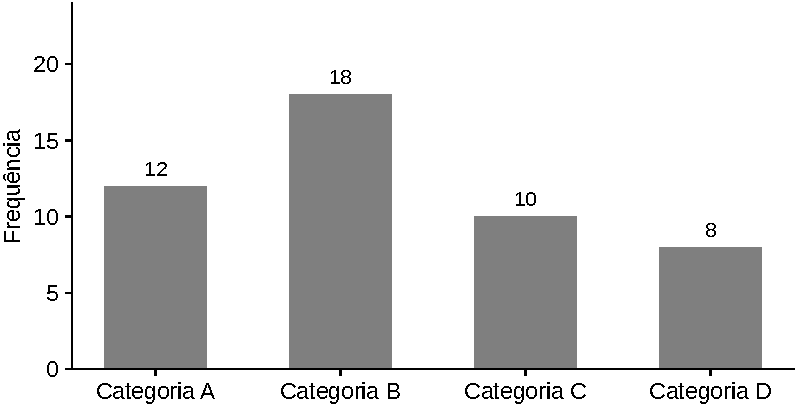
\includegraphics[width=\linewidth]{exemplo-grafico.pdf}
\fonte{Elaboração própria (\ano). Dados fictícios.}
\end{ilustracao}
\end{grafico}

\section{Resultados referentes ao segundo objetivo específico}
\label{sec:resultado2}

Equações e fórmulas são destacadas do texto e numeradas, quando necessário, para facilitar a remissão. A média aritmética, por exemplo, é dada pela Equação~\eqref{eq:media}:
% Equação destacada e numerada: ambiente equation, citada com \eqref.
% Símbolo no meio da frase: entre cifrões, como $n$.
\begin{equation}
\label{eq:media}
\bar{x} = \frac{1}{n}\sum_{i=1}^{n} x_i,
\end{equation}
em que $\bar{x}$ é a média, $n$ é o número de observações e $x_i$ é o valor da $i$-ésima observação.

\section{Discussão}
\label{sec:discussao}

% Relacione os resultados com o problema, os objetivos e a
% literatura apresentada na fundamentação teórica.
A discussão relaciona os resultados obtidos ao problema de pesquisa, aos objetivos e aos estudos apresentados na fundamentação teórica. Convém indicar em que medida os achados confirmam, ampliam ou divergem da literatura, sempre com a devida citação das fontes \cite{modeloartigo}, e apontar as possíveis explicações para as diferenças observadas.
